\section{Research Results}
\label{sec:research_results}
\lhead{\thesection \space Research Results}

The following chapter describes the results that the research brought forth. Structurally, the chapter is made up of sub-chapters detailing a list of various frameworks.
\newline
For each framework, it is described how the framework can be used to test a \textit{React Native} application. Furthermore, depending on the advantages and disadvantages the frameworks brings, it is defined whether or not the framework in question is fit to be used during the \textit{Connected.Football} project.
\newline
As far as the project itself is concerned, the developers work on a variety of operating systems, including \textit{Windows 10}, \textit{Gentoo Linux} and \textit{macOS 12 Mojave}, according to the interviews conducted with the developers. All developers furthermore deploy and test the application using an \textit{Android} based device or emulator. The developers would like the tests to make their work more efficient, by removing unnecessary repetition and navigation. Having additional unit tests to the end-to-end tests would also be an advantage (see \textit{Appendices \ref{appendix:interview_lucas_gehlen}, \ref{appendix:interview_marco_kull}, \ref{appendix:interview_patrick_richter}}).

\subsection{Jest}
\label{ssec:jest}

\textit{Jest} is the testing framework that is automatically installed whenever a new \textit{React Native} app is created. It is also developed by Facebook. Since version 14, \textit{Jest} is able to create so-called snapshots. Snapshots are records of how a certain part of an application rendered the last time the tests ran successfully. This means that to test using \textit{Jest}, it is defined what component is to be tested with certain properties. If this test has never run, the resulting component rendering tree is stored as a snapshot. If a snapshot already exists, the new rendering tree is compared against it, marking the differences to the snapshot. If the changes are intentional, the developer can store the result as a new snapshot. Ideally, these snapshots should always be committed and stored together with the sources. (\cite{testing-react-native})
\newline
The benefit to using \textit{Jest} is that it is completely platform-independent. What is tested is the generated \textit{React Native} rendering tree, rather that how the platform it is deployed on interprets it. Furthermore, the tests are not dependent on any emulation of an actual device: \textit{"Because tests are run in a command line runner instead of a real browser or on a real phone, the test runner doesn’t have to wait for builds, spawn browsers, load a page and drive the UI to get a component into the expected state which tends to be flaky and the test results become noisy."} (\cite{testing-react-native-with-jest})
\newline
Furthermore, due to not being dependent on a platform, it is also rather simple to provide information that is not accessible through other means, for instance through mocking. State, properties and other values can be given to the tests instead of having to simulate them. This has the advantage than rather to having to replicating state logic in the tests, this logic can also be tested. (\cite{learning-test-react-native})
\newline
However, despite the aforementioned advantages, \textit{Jest} is most useful when testing single components or at most somewhat high-level components. This makes it most useful for unit and component testing. End-to-end testing is rather hard to do with a framework that can only compare old versions of components to new ones. Ideally, \textit{Jest} would have to compare snapshots after executing a chain of commands that are processed by the application that is to be tested. This is also the reason why \textit{Jest} is used in a similar way in some of the testing frameworks mentioned below.

\subsection{Appium}
\label{ssec:appium}

\textit{Appium} is an end-to-end testing framework which uses \textit{Selenium} as a base. Since it was \textit{".. released even before React.js, [making it] the number one in the industry"} (\cite{detox-vs-appium}), it gathered a large following both of \textit{React Native} developers as well as developers using it in different environments. Similar to \textit{Detox}, it makes use of a selection API which sends inputs to specified parts of the application, which is running in an emulator. \textit{Appium} is also able to run tests on actual devices. If an \textit{Android} device is connected to the development machine, \textit{"providing there is only a single device connected, the test will pick up that device for execution."} (\cite[p. 169]{test-automation-appium})
\newline
To run \textit{Appium}, a service is started which connects to the emulator. This service is responsible for propagating the inputs to the actual app. The service itself is actually an HTTP server, as seen in \textit{Figure \ref{fig:appium_server}}, developed in \textit{Node.js} which creates \textit{WebDriver} sessions (\cite{appium-and-selenium}). These sessions can be used by client applications which use certain drivers, depending on the programming language the tests are written in. To test the project in question, the tests are written in \textit{JavaScript}, just like the actual application is. The driver that was made use of is \textit{Webdriver.IO} which comes with its own selection API (\cite{webdriverio}).

\begin{figure}[H]
    \begin{center}
        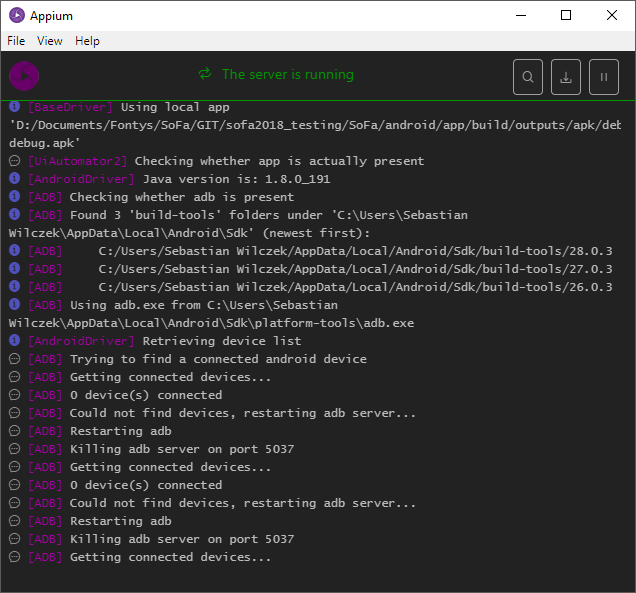
\includegraphics[width=0.9\textwidth]{images/appium_server.png}
        \caption{\textit{Appium} Server}
        \label{fig:appium_server}
    \end{center}
\end{figure}

\newpage

Defining tests in \textit{Appium} is simple. As seen in \textit{Listing \ref{lst:appiumTest}}, test cases can be described which in turn contain instructions on how to interact with the application, or rather how the \textit{Appium} service should interact, including setup and tear down functions to start and end sessions with the service. The actual definition of interaction can make use of the driver's selection API. In the case of testing with \textit{Appium}, this selection is limited to so-called \textit{Accessibility Labels}. These labels are defined in the \textit{React Native} source code and can be read in an \textit{Appium} test using the '\textit{\~}' character

\begin{lstlisting}[language=javascript,caption=\textit{Appium WebdriverIO} Test Example,label=lst:appiumTest]
describe("Basic Android interactions", function() {
  let client;

  beforeEach(function() {
    client = webdriverio.remote(opts);
    return client.init().pause(15000);
  });

  afterEach(function() {
    return client.end();
  });

  it("should click a tab that opens more functionality", async function() {
    return client
      .waitForExist('~More', 5000)
      .element('~More')
      .click()
      .waitForExist("~Privacy", 5000)
      .getText("~Privacy", function(result) {
        assert.equal(result.value, "Privacy");
      });
  });
});
\end{lstlisting}

Using the labels has two major downsides. First of all, the development team would be forced to create such an identification for each element that would be involved in the testing process. As stated in the interviews, it would be preferable to test using as little change to actual developed work as necessary.
\newline
Furthermore, the \textit{Accessibility Label} is also exposed to the user. In the accessibility options of \textit{Android}, it is possible to enable a setting that enables screen reading applications to read out the functions of an application to vision-impaired users, as described by the aforementioned labels. (\cite{accessible-apps})
\newline
Unfortunately, the labels are also the reason why the testing framework can not be applied to the project in question. While it was possible to define and execute tests using \textit{Appium}, including interacting with the application, the application also makes use of various open source \textit{React Native} components which do not support the usage of \textit{Accessibility Labels}. In particular, the module \textit{react-native-navigation} caused problems this way, making it impossible for tests to ever leave the starting view of the application.

\subsection{Espresso}
\label{ssec:espresso}

\textit{Espresso} is a library developed and maintained by Google designed for \textit{Android} test automation (\cite{appium-pro}). Since it is developed only for \textit{Android}, it can not be used to test applications running on an \textit{iOS} device or emulator.
\newline
The testing framework was developed having \textit{Android} native applications in mind, with the possibility of testing \textit{React Native} applications added later on. Given this change, \textit{Espresso} was also made available to be used as a driver for \textit{Appium}, similar to \textit{Webdriver.IO} and \textit{UIAutomator2}, which is also developed by Google.
\newline
An advantage of using \textit{Espresso} is the way it manages timing while interacting with the application. \textit{"Espresso requires no waiting method calls to ensure synchronization of the UI, [making it] clearly [one of] the fastest of the tools"} (\cite{comparison-gui}).
\newline
However, in the same way as \textit{Appium}, the framework is only able to access components through given identification, which is again defined through labels. This again makes it impossible to use \textit{Espresso} in the given project. For detailed information about the problem posed by the \textit{Accessibility Labels}, see \textit{Chapter \ref{ssec:appium} \nameref{ssec:appium}}.

\subsection{Detox}
\label{ssec:detox}

\textit{Detox} is another testing framework that simulates user interaction. Originally it was developed to run only on \textit{macOS} and \textit{iOS} platforms. Recently, the developers decided to make the framework available to \textit{Android} developers as well, releasing in-development artefacts as they are continuing to make it fully functional. (\cite{android-status})
\newline
Similar to \textit{Espresso}, \textit{Detox} tries to improve test stability using a gray box approach, by only running interactions once other interactions have been processed and the application is running in an idle state. \textit{Figure \ref{fig:detox_check}} shows the check performed by \textit{Detox} every few milliseconds. The framework will wait until it is asserted that the application's resources are running in an idle state or until a callback makes \textit{Detox} run regardless.

\begin{figure}[H]
    \begin{center}
        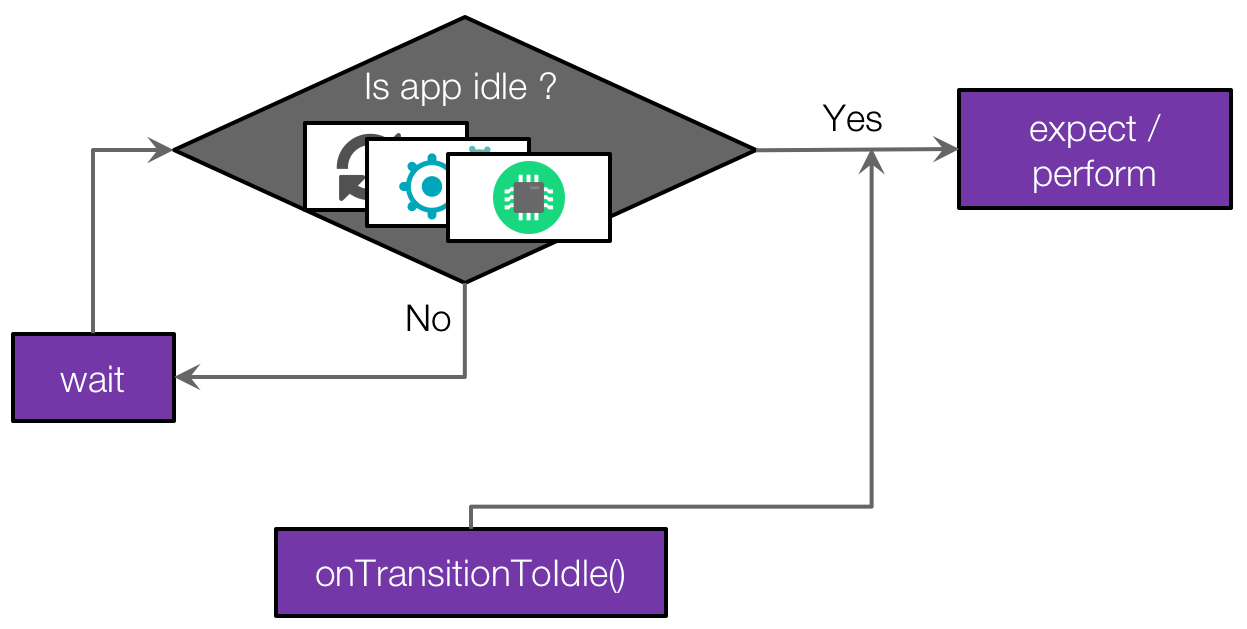
\includegraphics[width=0.8\textwidth]{images/detox_check.png}
        \caption{\textit{Detox} Idle State Check (\cite{detox-gray-box})}
        \label{fig:detox_check}
    \end{center}
\end{figure}

\newpage

\textit{Detox} is very simple to setup and use in a project. Once it has been installed as part of the modules of a \textit{React Native} project, multiple configurations can be created to test in different environments, such as different devices running \textit{Android} and \textit{iOS}. \textit{Listing \ref{lst:detoxConfig}} shows two such configurations.

\begin{lstlisting}[language=json,caption=\textit{Detox} Configuration Example,label=lst:detoxConfig]
"detox": {
  "configurations": {
    "ios.sim.debug": {
      "binaryPath": "ios/build/Build/Products/Debug-iphonesimulator/example.app",
      "build": "xcodebuild -project ios/example.xcodeproj -scheme example -configuration Debug -sdk iphonesimulator -derivedDataPath ios/build",
      "type": "ios.simulator",
      "name": "iPhone 7"
    },
    "android.emu.debug": {
      "binaryPath": "android/app/build/outputs/apk/debug/app-debug.apk",
      "build": "cd android && gradlew assembleDebug assembleAndroidTest -DtestBuildType=debug && cd ..",
      "type": "android.attached",
      "name": "emulator_5554"
    }
  },
  "test-runner": "jest"
}
\end{lstlisting}

These configurations include definitions on how to run the test builds as well as on what platform to run them. For instance, the second configuration run the test using ADB on an \textit{Android} device with the name \textit{emulator\_5554}, which in this case is the running AVD emulator.
\newline
Just like most other frameworks, \textit{Detox} has an API to select components. However, there is at the time of writing no documentation that details how this API can be used with a \textit{React Native} application that is built for and deployed to an \textit{Android} device. It could however be assumed that it might have to rely on \textit{Accessibility labels}, just like \textit{Appium}.
\newline
Furthermore, when trying to run an example test, just to see if it fails, \textit{Detox} failed to run with multiple different errors depending on the chosen configuration. No documentation or reproduction of these errors could be found either. It is not known if the low support and early development stage of the \textit{Android} functionality or the compatibility to the given project is to blame, however, the high amount of errors with no apparent solution makes \textit{Detox} unsuitable for the project, despite being a promising product.

\subsection{Cavy}
\label{ssec:cavy}

\textit{Cavy} is the newest available framework to test \textit{React Native} applications at the time of writing. It tests applications by running an application in a simulated environment, in the same way \textit{Appium} and \textit{Detox} does, finding components using a selection API and interacting with them in a specified way.
\newline
The difference between \textit{Cavy} and other similar tools is the way it finds and accesses components. The most notable \textit{".. difference is that Appium uses native hooks to access components (accessibility IDs), wheras [sic] Cavy uses React Native refs. This means that Cavy sits directly within your React Native environment [...] without much overhead."} (\cite{cavy})
\newline
While it is a good idea to use only functionality that is already available in the \textit{React Native} framework, this also means that every component that has to be tested has to be marked as such. To do so, \textit{"Cavy (ab)uses React ref generating functions to give you the ability to refer to, and simulate actions upon, deeply nested components within your application."} (\cite{cavy})
\newline
In other terms, that means that every component written in \textit{React Native} needs to include a specific syntax when used. This syntax appears to be rather complicated, as shown in \textit{Listing \ref{lst:cavyHook}}, and can become hard to read when used in many components.

\begin{lstlisting}[language=javascript,caption=\textit{Cavy} Hook Example,label=lst:cavyHook]
<TextInput
  ref={this.props.generateTestHook('Scene.TextInput')}
  onChangeText={...}
/>
\end{lstlisting}

There is a small workaround available to make the source code more readable. This workaround makes use of \textit{Higher-Order Components}, which \textit{"is an advanced technique in React for reusing component logic"} (\cite{hoc}). Making use of this technique, the rather complex looking syntax can be replaced by the word \textit{testable} and the name of the components to be referenced with. Essentially this is the same as the previous syntax, just far more readable. (\cite{e2e_cavy})
\newline
In any case, the entire app must also be wrapped in a test related component, which receives the testing hooks. This another change to production code that is undesirable.
\newline
While the creation of test hooks looks rather complicated, the definition of tests is rather simple. The selection API provides, even if it is a bit simplistic, enough ways to select and interact with \textit{React Native} components. An example test script can be found in \textit{Listing \ref{lst:cavyTest}}.

\begin{lstlisting}[language=javascript,caption=\textit{Cavy} Test Example,label=lst:cavyTest]
export default function(spec) {
  spec.describe('My feature', function() {
    spec.it('works', async function() {
      await spec.fillIn('Scene.TextInput', 'some string')
      await spec.press('Scene.button');
      await spec.exists('NextScene');
    });
  });
}
\end{lstlisting}

While \textit{Cavy} looks great in theory, aside from the massive change to the existing source code, it is not possible to make use of it in the project in question. The project makes heavy use of functional components, and since \textit{"functional components cannot be assigned a ref since they don't have instances"} (\cite{cavy}), \textit{Cavy} will not be able to access these components. Using \textit{Recompose}, it might be possible to convert functional components to \textit{React Native} classes, however that is more change to existing code and goes against the principle and goal of functional components.